\documentclass[aspectratio=169]{beamer}

\usetheme{Madrid}
\usecolortheme{default}

\usepackage[T1]{fontenc}
\usepackage[utf8]{inputenc}
\usepackage{lmodern}
\usepackage{amsmath,amssymb}
\usepackage{graphicx}
\usepackage{booktabs}
\usepackage{tabularx}

\graphicspath{{figures/}{./}}

\title[AI-Ready HAPS--UAV Channel Model]{An AI-Ready Air-to-Ground Channel Model for HAPS--UAV Access Networks}
\author{Harsha Matadhikari}
\institute{Online PG Diploma in Advanced Communication Engineering with Quantum AI Integration \\ Indian Institute of Technology Delhi}
\date{}

\begin{document}

% ---------------------------------------------------------------
\begin{frame}
\titlepage
\end{frame}

% ---------------------------------------------------------------
\begin{frame}{Motivation}
\begin{itemize}
  \item A 3-HAPS equilateral-triangle constellation serves a ground footprint via
        \textbf{service} (2\,GHz), \textbf{backhaul} (38\,GHz), and two-hop
        \textbf{UAV relay} links.
  \item Distance-only link budgeting misses a key effect: co-channel
        interference from the other two HAPS makes SINR depend strongly on
        \emph{angular position}, not just distance.
  \item Static link-quality analysis cannot react to this, or to
        time-varying rain fades on the 38\,GHz backhaul.
  \item \textbf{AI Ready Model:} a validated channel model, an LSTM rain
        forecaster, and a DQN agent that learns real-time user--platform
        association.
\end{itemize}

\vspace{4mm}
\begin{center}
\footnotesize
\textbf{Research flow:}\\[1mm]
\fbox{\parbox{0.27\textwidth}{\centering Attenuation \& channel models\\(FSPL, rain, fog, gas, scintillation, interference)}}
$\;\rightarrow\;$
\fbox{\parbox{0.22\textwidth}{\centering Baseline policies\\(random, max-SINR, max-throughput)}}
$\;\rightarrow\;$
\fbox{\parbox{0.27\textwidth}{\centering AI model\\(LSTM forecast + DQN) for\\platform selection \& positioning}}
\end{center}
\end{frame}

% ---------------------------------------------------------------
\begin{frame}{System Topology and Channel Model}
\begin{columns}[T]
\begin{column}{0.5\textwidth}
\vspace{-11mm}
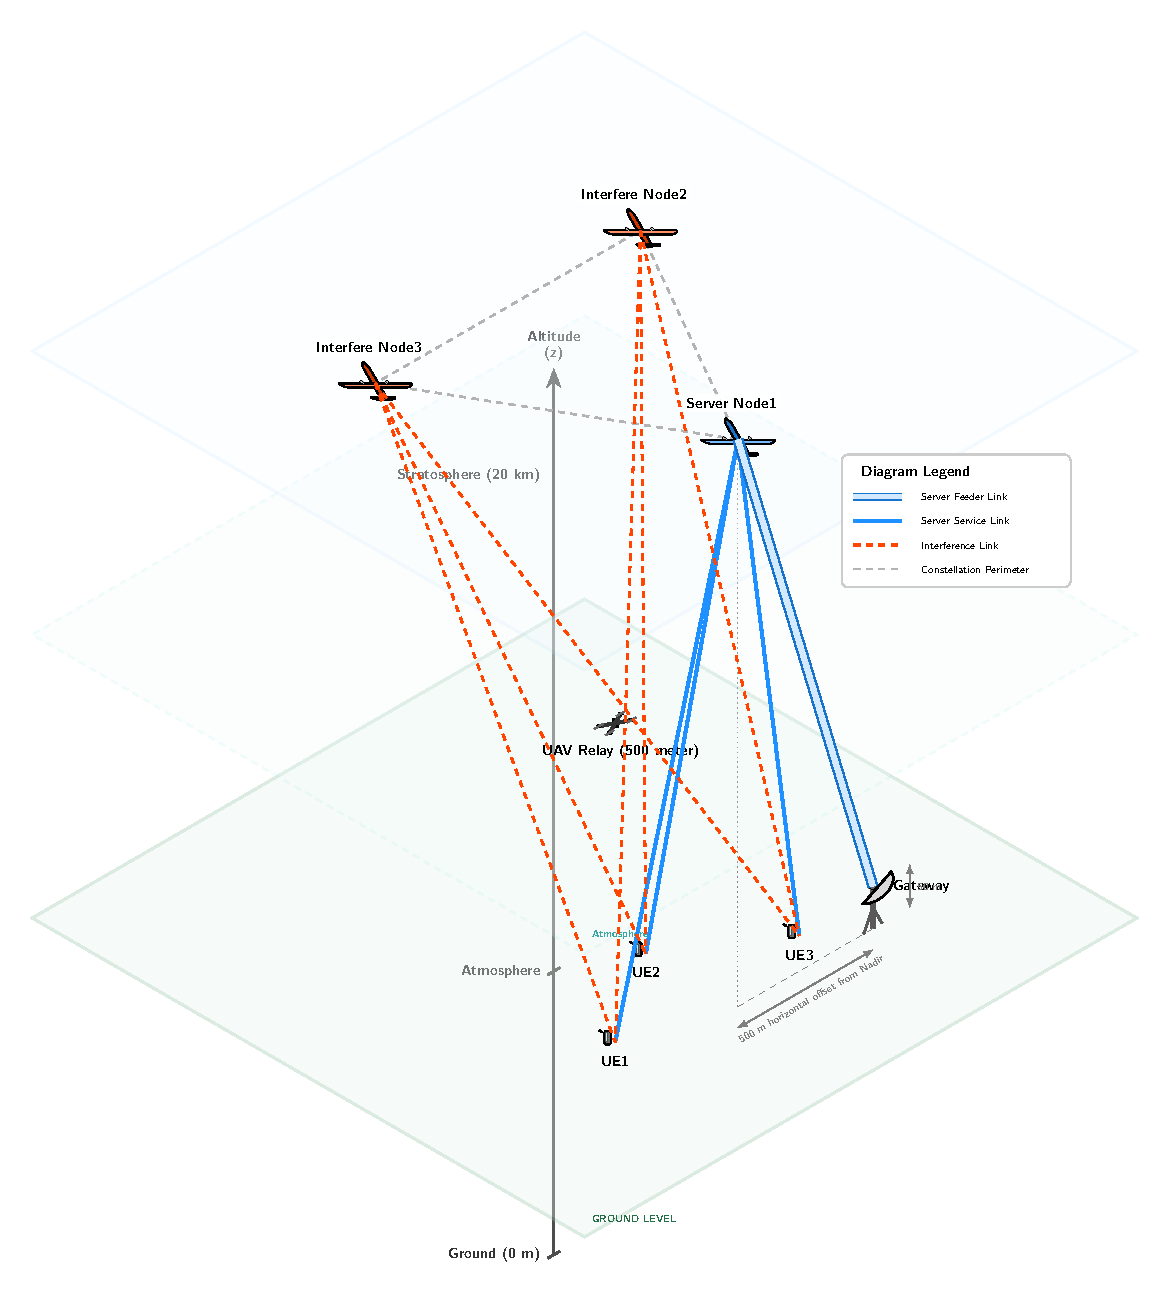
\includegraphics[width=\linewidth]{network_diagram.pdf}
\end{column}
\begin{column}{0.5\textwidth}
\footnotesize
\textbf{Three link types:}
\begin{itemize}
  \item HAPS $\rightarrow$ UE (service, 2\,GHz)
  \item HAPS $\rightarrow$ Gateway (backhaul, 38\,GHz)
  \item HAPS $\rightarrow$ UAV $\rightarrow$ UE (relay; feeder hop at
        38\,GHz, UAV$\rightarrow$UE access hop at 2\,GHz)
\end{itemize}
\vspace{4mm}
\textbf{Channel model:}
\begin{itemize}
  \item Free-space path loss (HAPS tier)
  \item Building-blockage LoS/NLoS probability (UAV tier, Holis \& Pechac 2008)
  \item ITU-R rain, fog, gas, and scintillation losses (backhaul/feeder)
\end{itemize}
\end{column}
\end{columns}
\end{frame}

% ---------------------------------------------------------------
\begin{frame}{Path Loss and SINR vs.\ Distance}
\begin{columns}[T]
\begin{column}{0.34\textwidth}
\centering
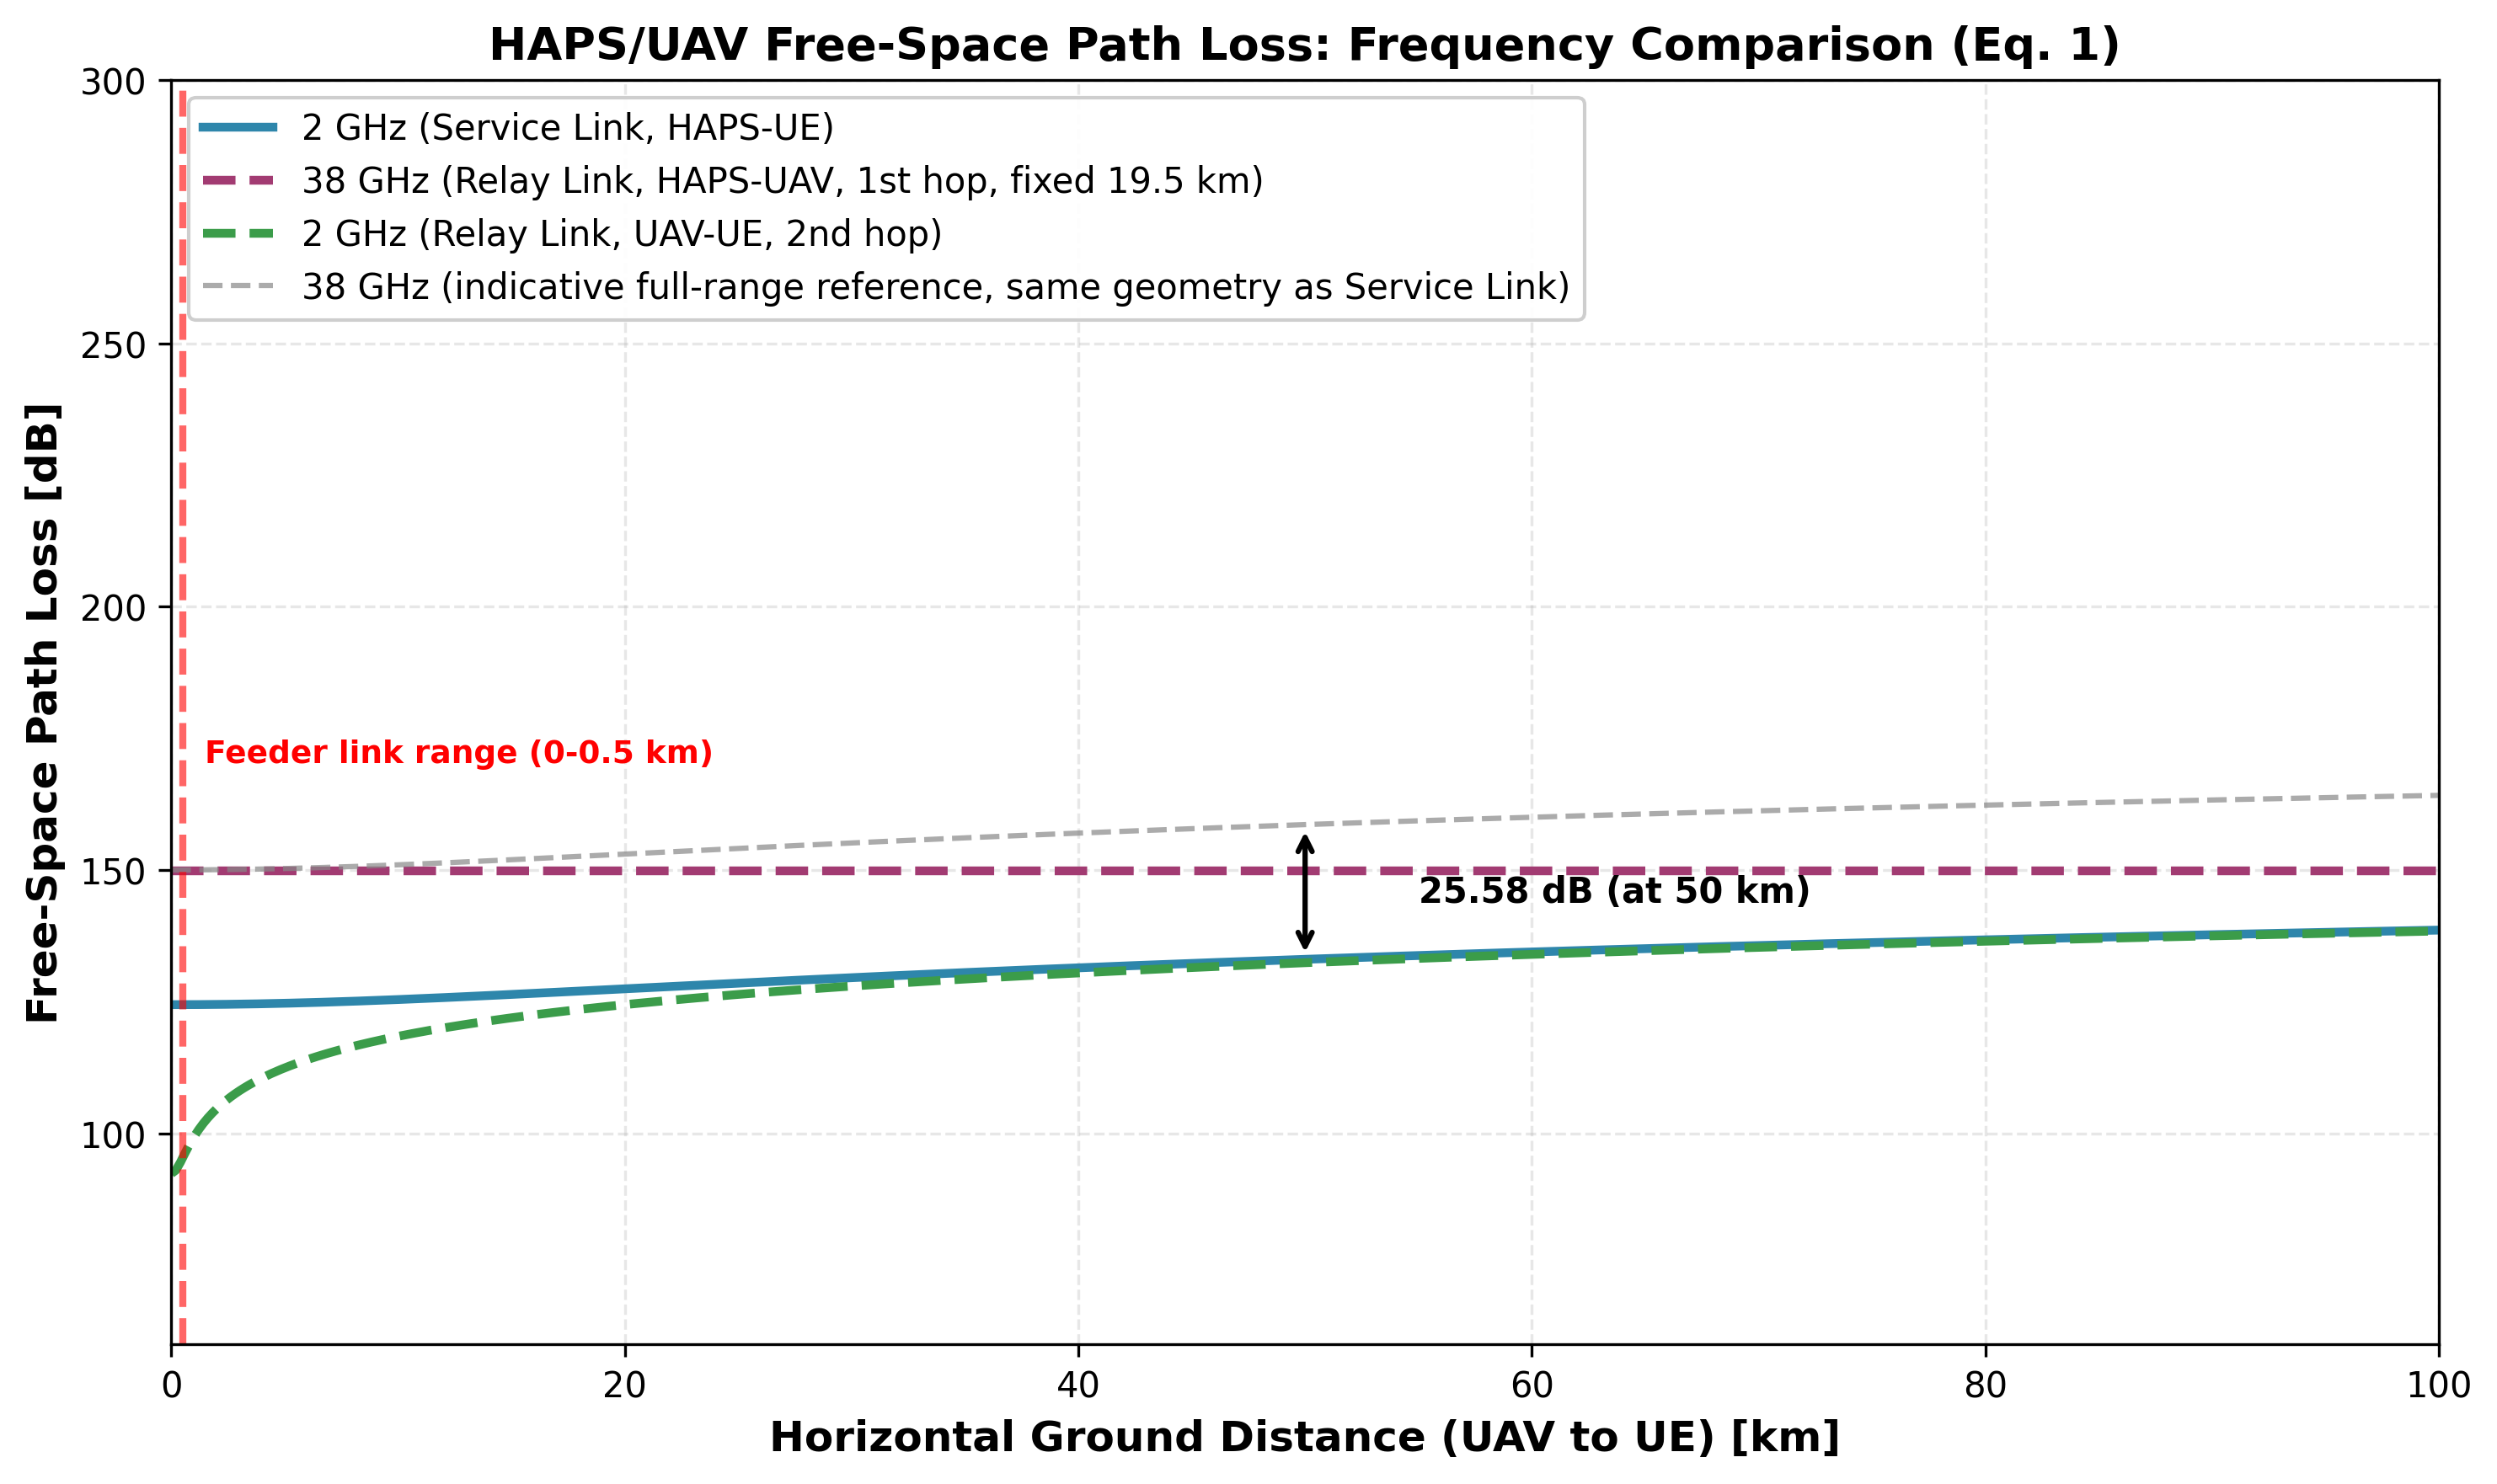
\includegraphics[width=\linewidth]{1b_haps_fspl_2ghz_vs_38ghz.png}\\
\scriptsize\textbf{FSPL vs.\ distance} -- same form for 2\,GHz and
38\,GHz; the feeder sits $\approx$25.6\,dB higher purely from the
frequency term.
\end{column}
\begin{column}{0.33\textwidth}
\centering
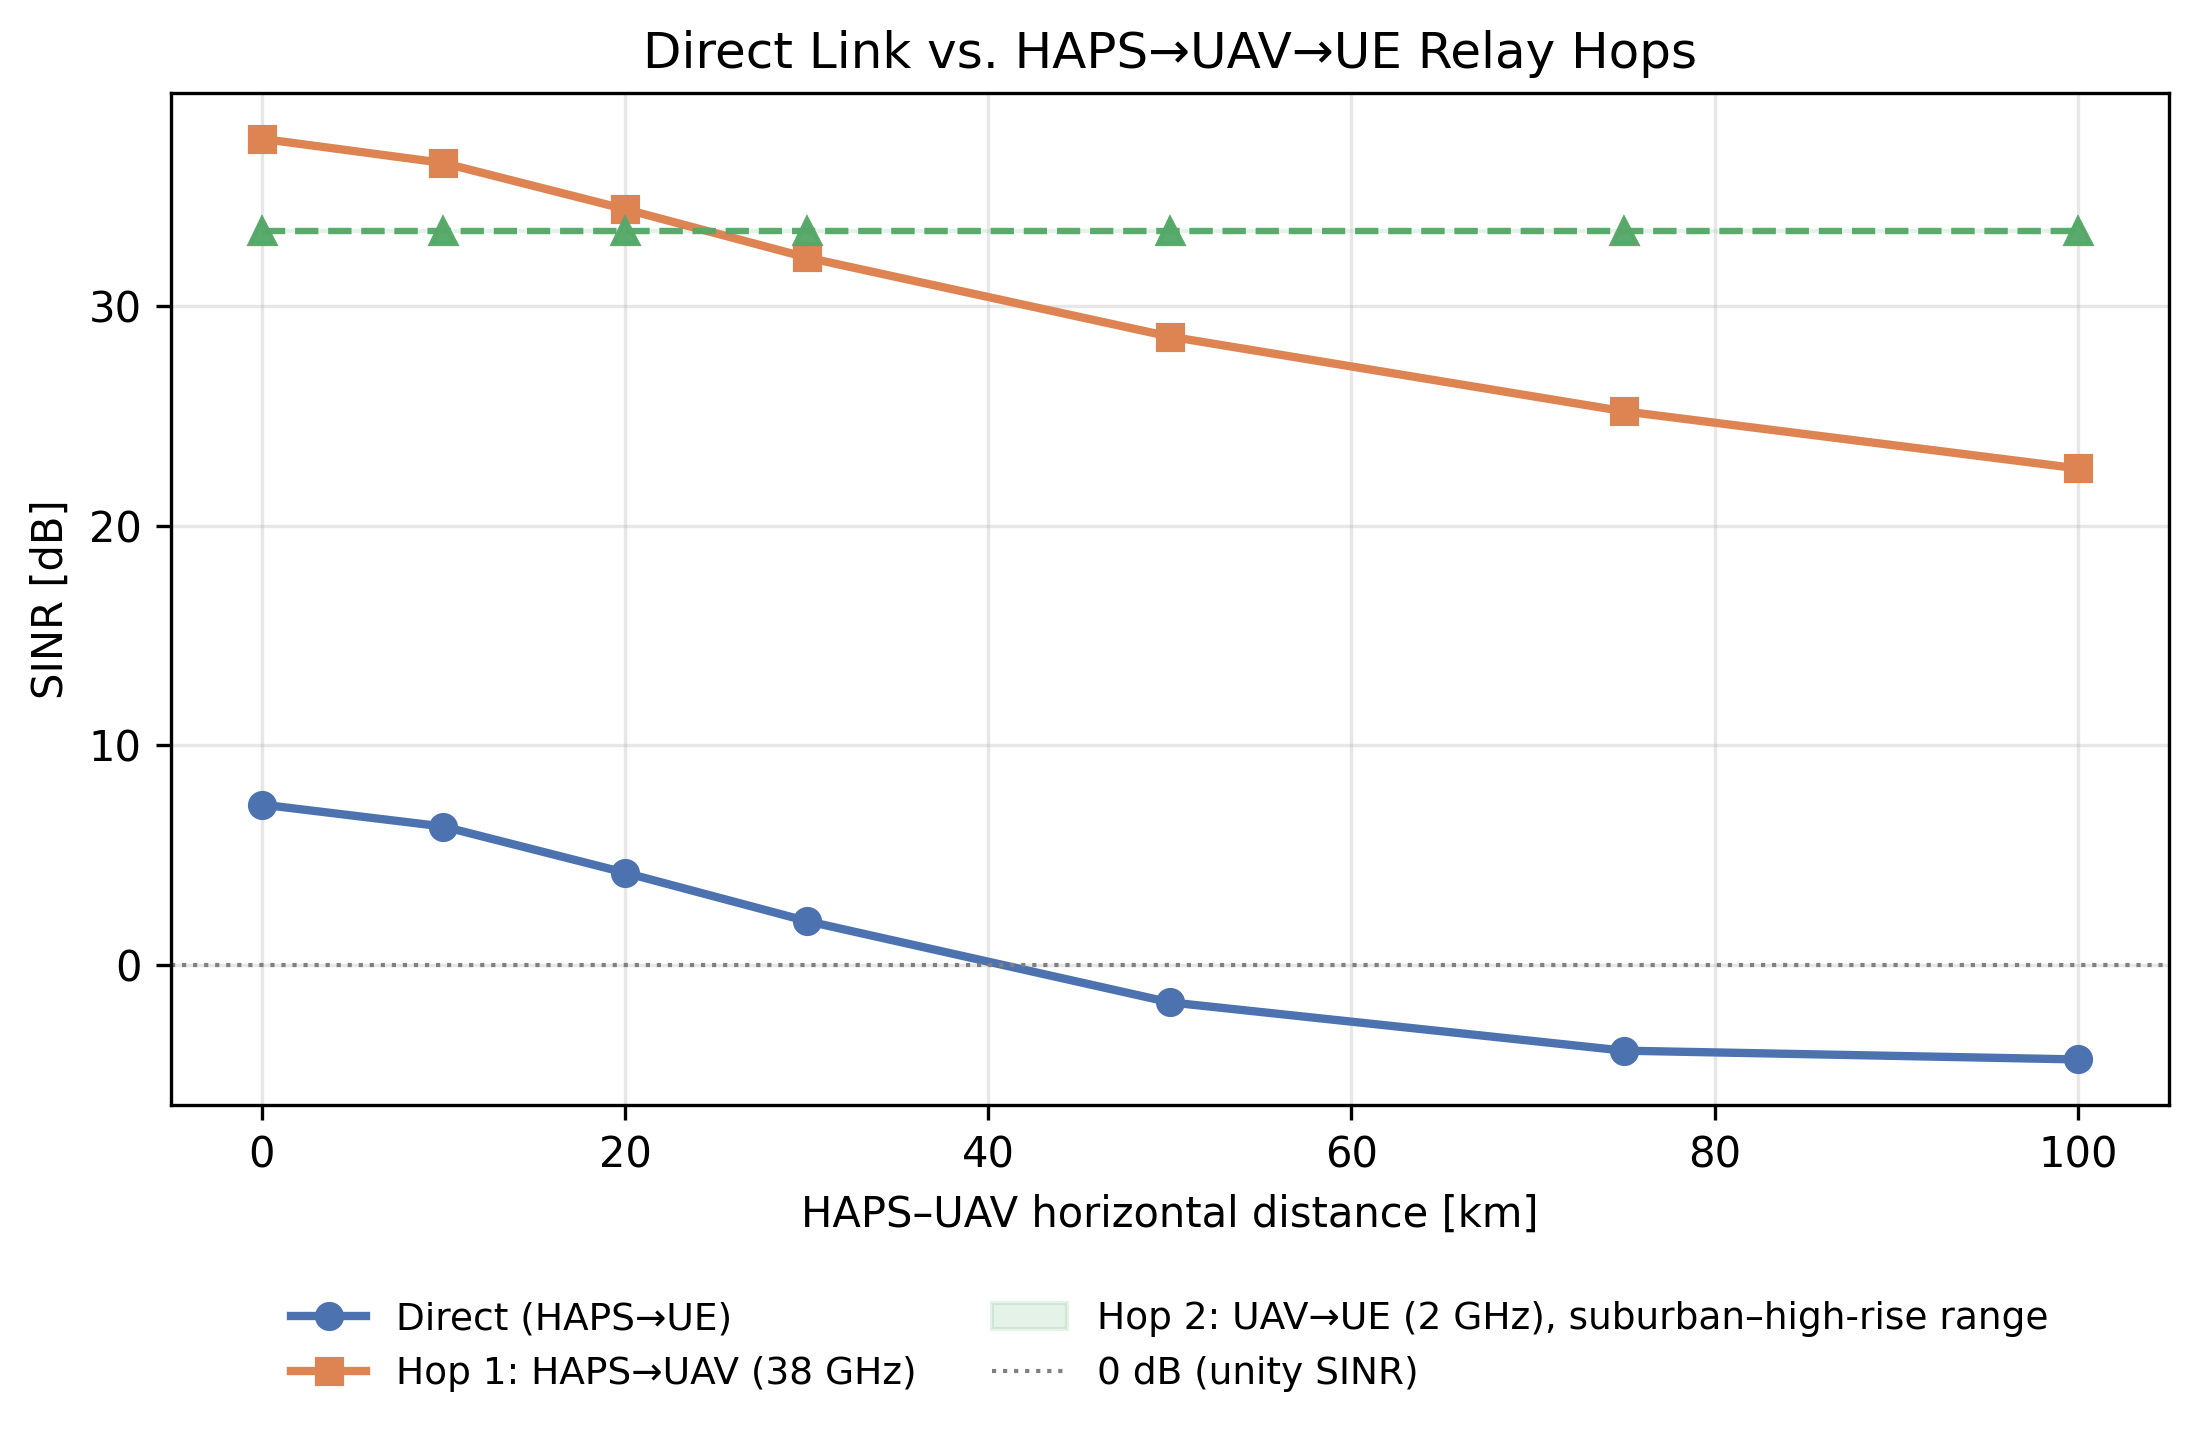
\includegraphics[width=\linewidth]{12_uav_relay_comparison.png}\\
\scriptsize\textbf{SINR vs.\ distance} -- direct link falls below
0\,dB past $\approx$40\,km, while both relay hops (feeder 38\,GHz,
access 2\,GHz) stay well above it at every distance tested.
\end{column}
\begin{column}{0.33\textwidth}
\centering
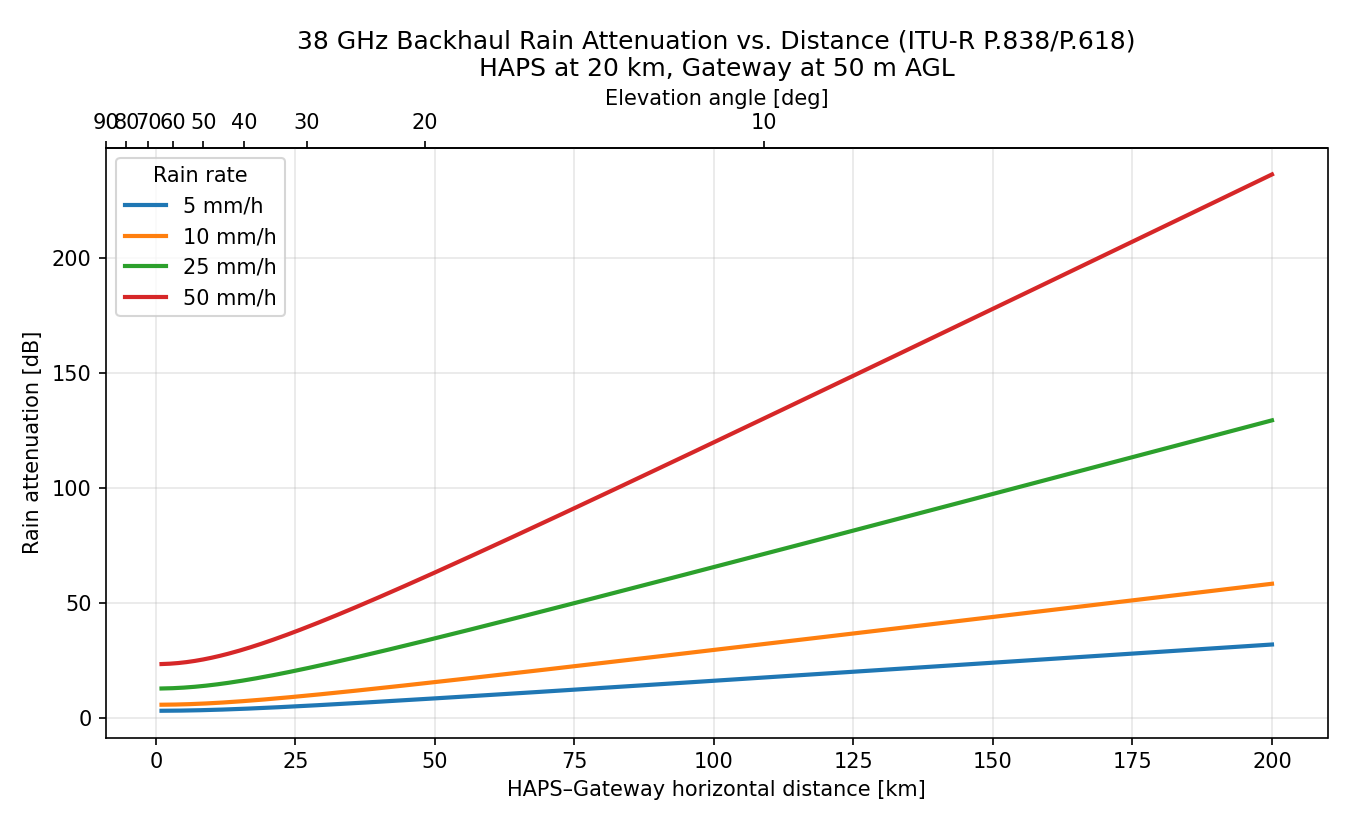
\includegraphics[width=\linewidth]{rain_attenuation_vs_distance.png}\\
\scriptsize\textbf{Rain attenuation vs.\ distance} (38\,GHz backhaul)
-- grows faster than linear past $\approx$100\,km as elevation drops
and the rain slant-path lengthens.
\end{column}
\end{columns}
\end{frame}

% ---------------------------------------------------------------
\begin{frame}{Why 38\,GHz: Frequency Selection}
\begin{columns}[T]
\begin{column}{0.48\textwidth}
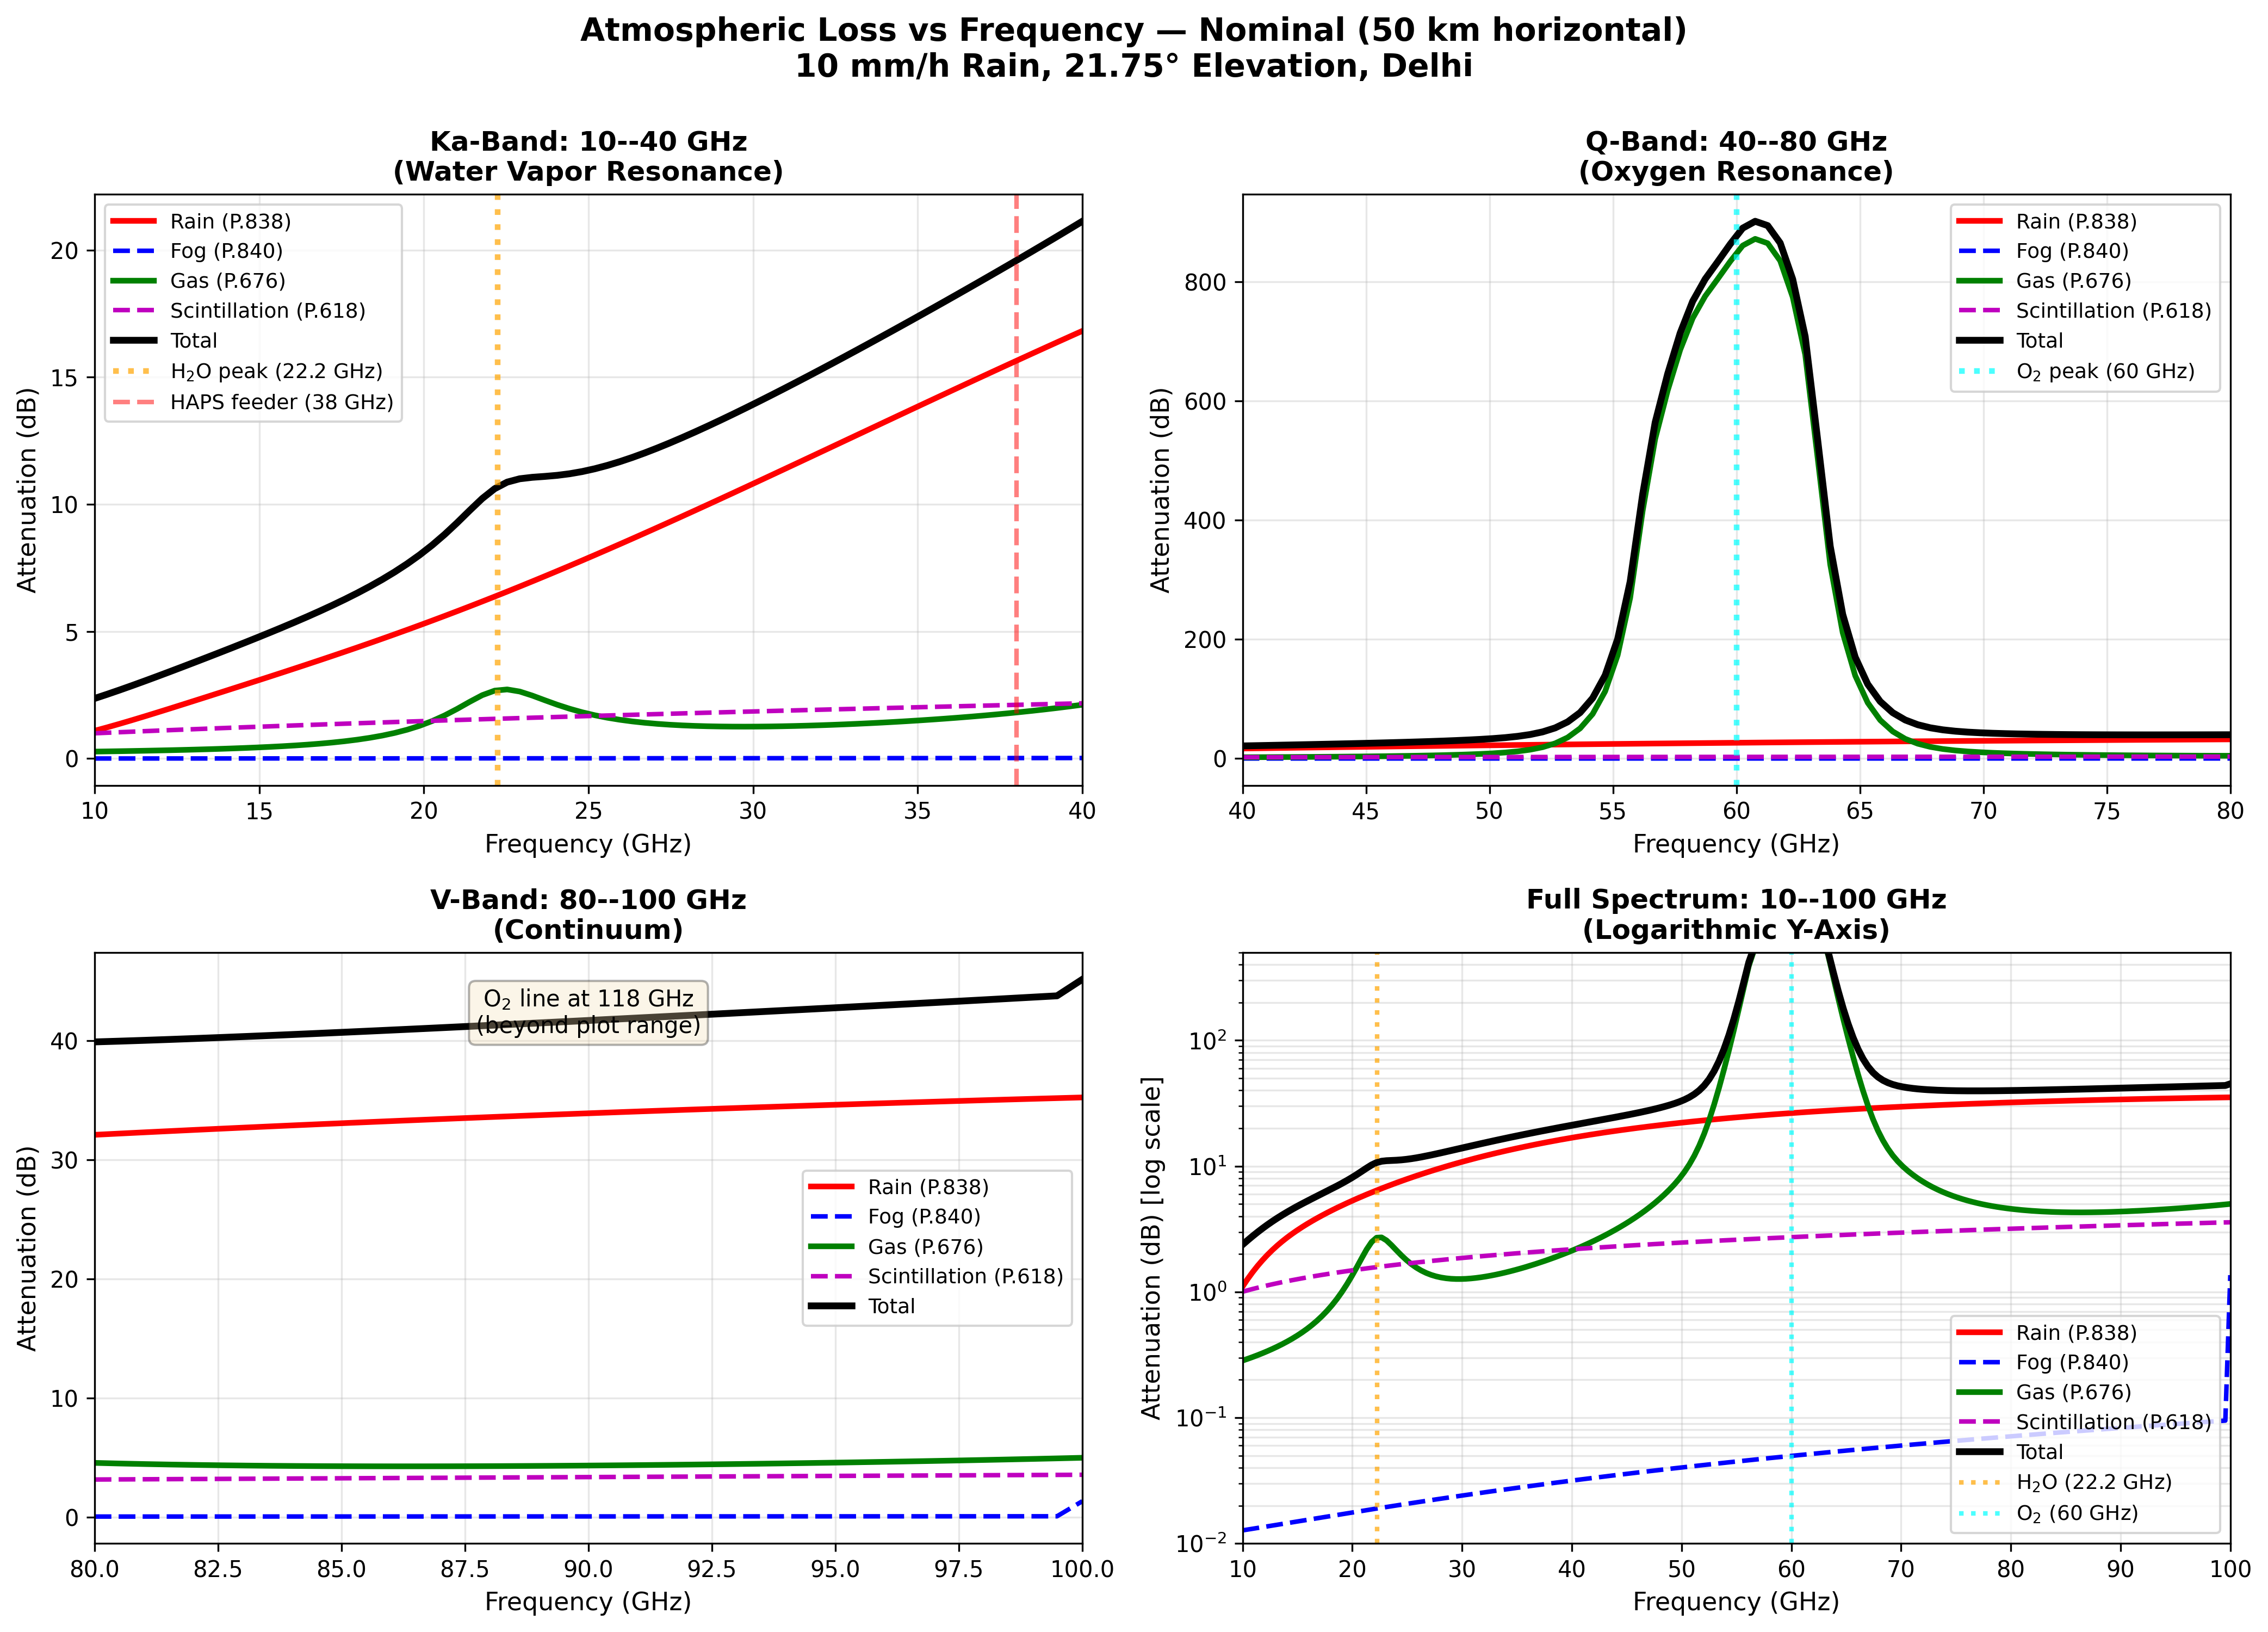
\includegraphics[width=\linewidth]{fig_atm_loss_nominal_frequency.png}
\end{column}
\begin{column}{0.52\textwidth}
\footnotesize
Atmospheric loss (rain, fog, gas) swept across the Ka/Q/V bands for
the Delhi gateway path, 10\,mm/h rain:
\begin{itemize}\setlength{\itemsep}{2pt}
  \item \textbf{Rain} (P.838/P.618) -- dominant term, grows roughly
        linearly with frequency; up to $\approx$19\,dB at 99.9\%
        availability ($R_{0.1}=15.7$\,mm/h).
  \item \textbf{Fog/cloud} (P.840) -- small except in dense fog;
        negligible below 10\,GHz.
  \item \textbf{Gas absorption} (P.676) -- two resonance peaks to
        avoid: H$_2$O at 22.2\,GHz, O$_2$ at 60\,GHz (there, total
        loss exceeds 800\,dB over 50\,km -- unusable).
\end{itemize}
\textbf{38\,GHz sits in the valley} between these peaks
($\approx$0.2--0.3\,dB/km clear-sky gas loss) -- this, not just
available bandwidth, is why it was chosen over a frequency closer to
either resonance.
\end{column}
\end{columns}
\end{frame}

% ---------------------------------------------------------------
\begin{frame}{Angular Interference Sectors and Scintillation Fading}
\begin{columns}[T]
\begin{column}{0.48\textwidth}
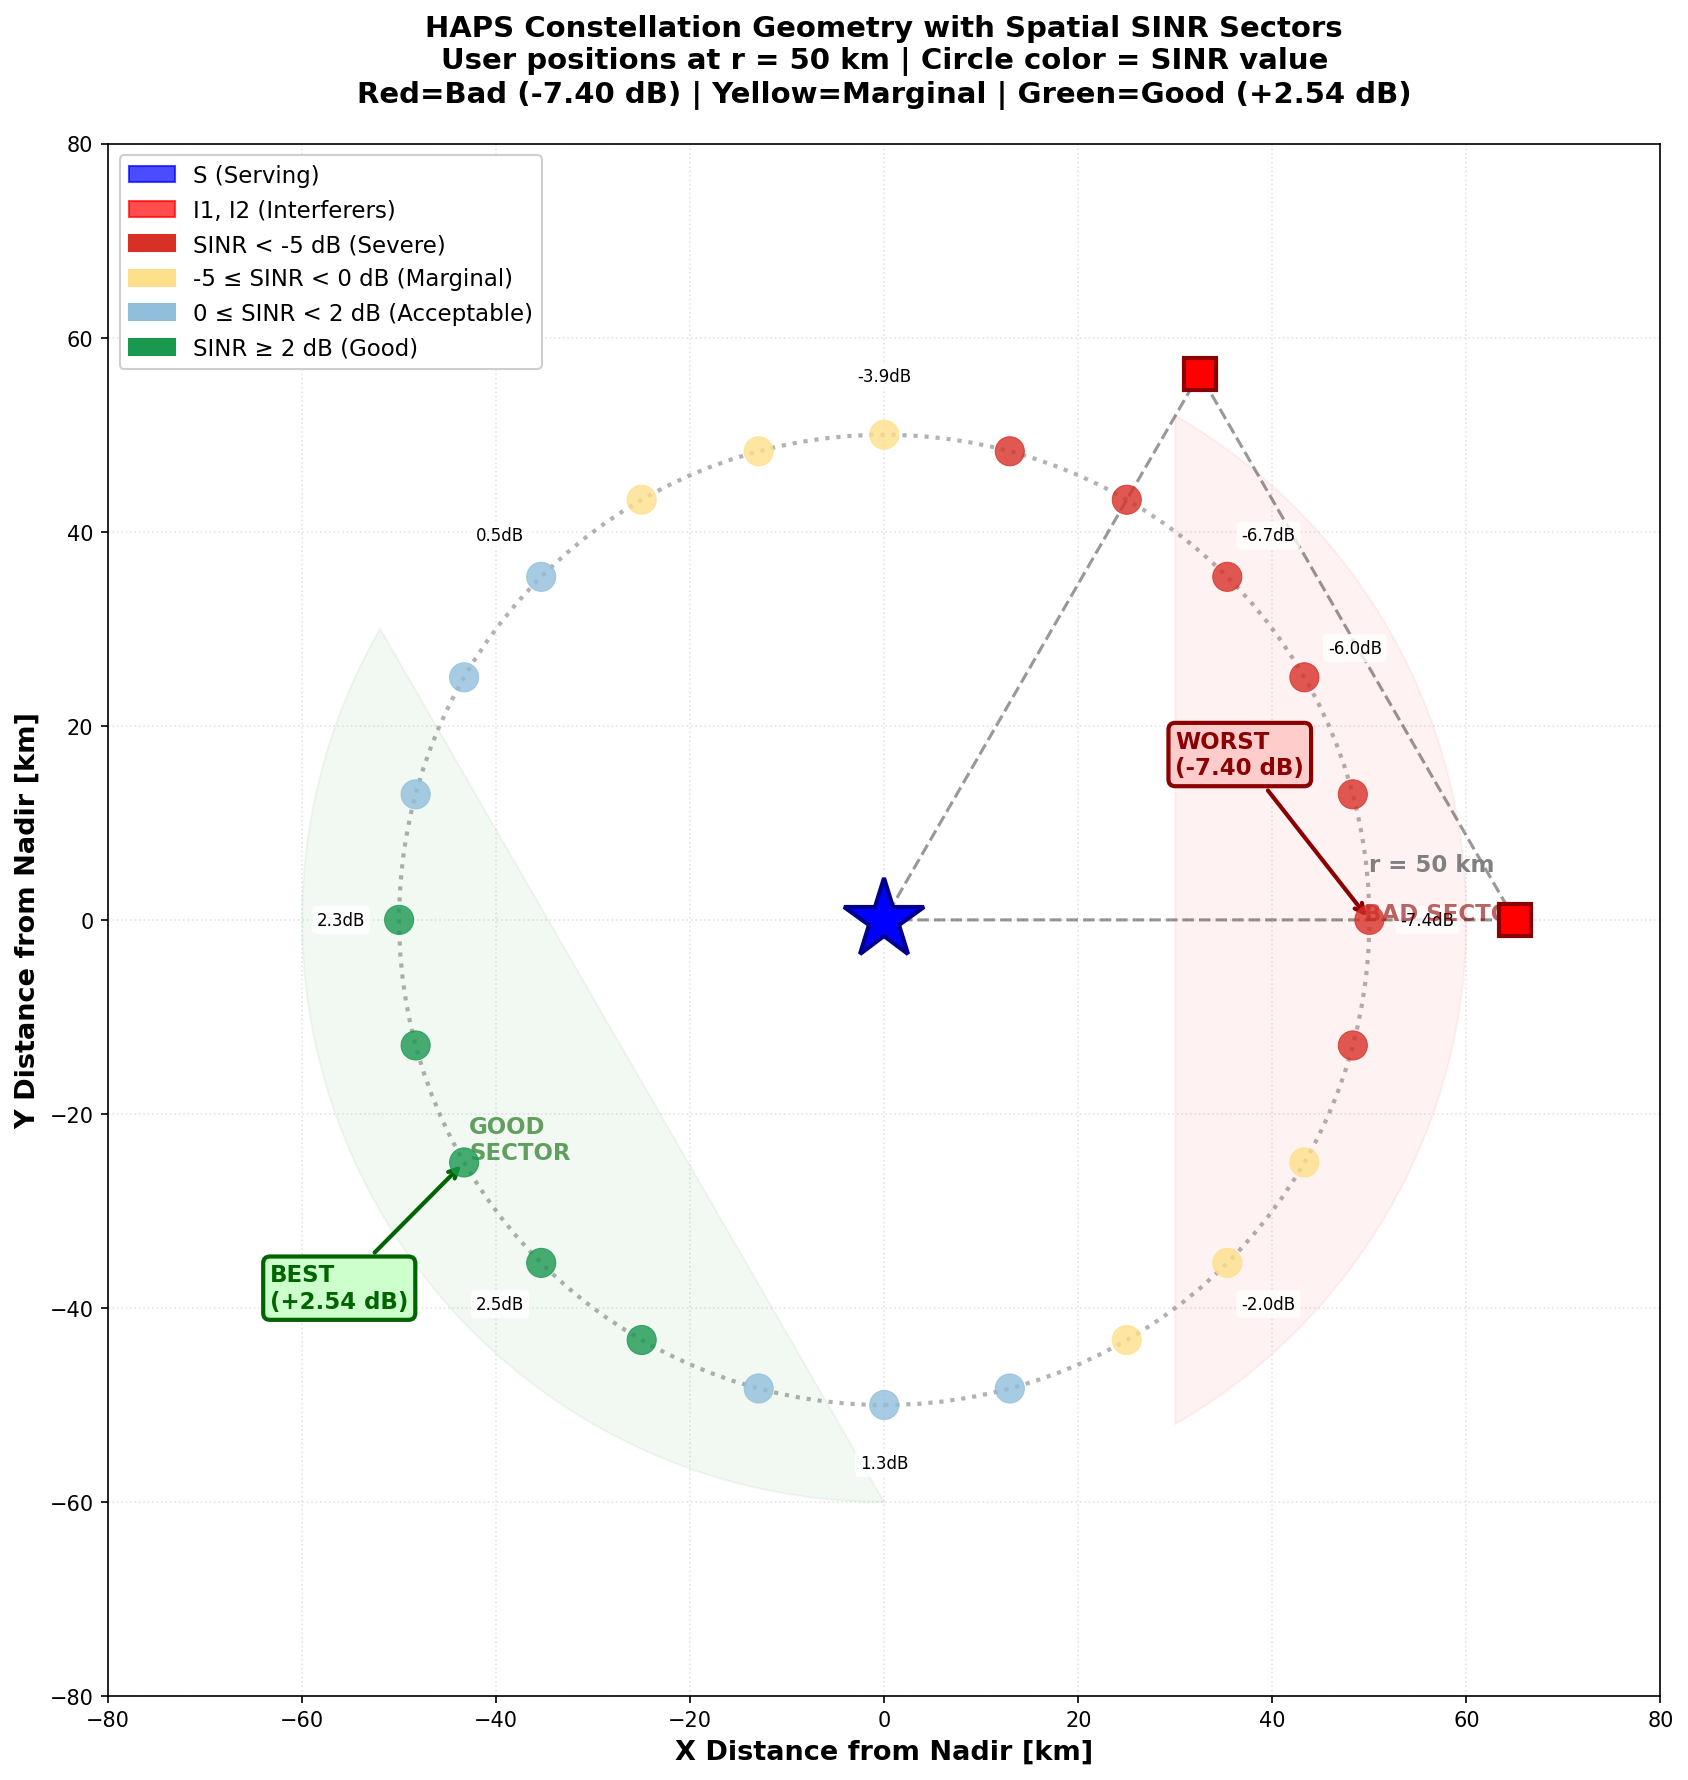
\includegraphics[width=\linewidth]{constellation_with_sectors.png}
\end{column}
\begin{column}{0.52\textwidth}
\footnotesize
\textbf{Angle-dependent SINR (sectors):} the 3-HAPS triangle creates a
good sector ($\approx$120\textdegree--290\textdegree, away from
interferers) and a bad sector ($\approx$330\textdegree--75\textdegree,
toward them) -- same radius, up to 9.94\,dB apart.

\vspace{2mm}
\textbf{Scintillation (ITU-R P.618):} rapid amplitude fluctuations
from tropospheric turbulence; grows with frequency, shrinks with
elevation. At 30\textdegree\ elevation, $p=0.01\%$: $\approx$0.49\,dB
at 38\,GHz vs.\ $\approx$0.09\,dB at 2.1\,GHz.

\vspace{2mm}
Favors positioning the UAV relay near nadir (higher elevation) when
feasible, especially for the HAPS--UAV feeder hop -- which also tends
to be away from the interferer-facing sector.

\vspace{2mm}
\scriptsize\textbf{Nuance:} each HAPS could simultaneously be a \emph{serving}
node (near-nadir, low-loss for its own users) and an \emph{interferer}
for the other two HAPS' users -- so this isn't a single clean
optimization across the constellation (future work, see Conclusion).
\end{column}
\end{columns}
\end{frame}

% ---------------------------------------------------------------
\begin{frame}{Why Learning is Needed: Spatial SINR Heterogeneity}
\begin{columns}[T]
\begin{column}{0.55\textwidth}
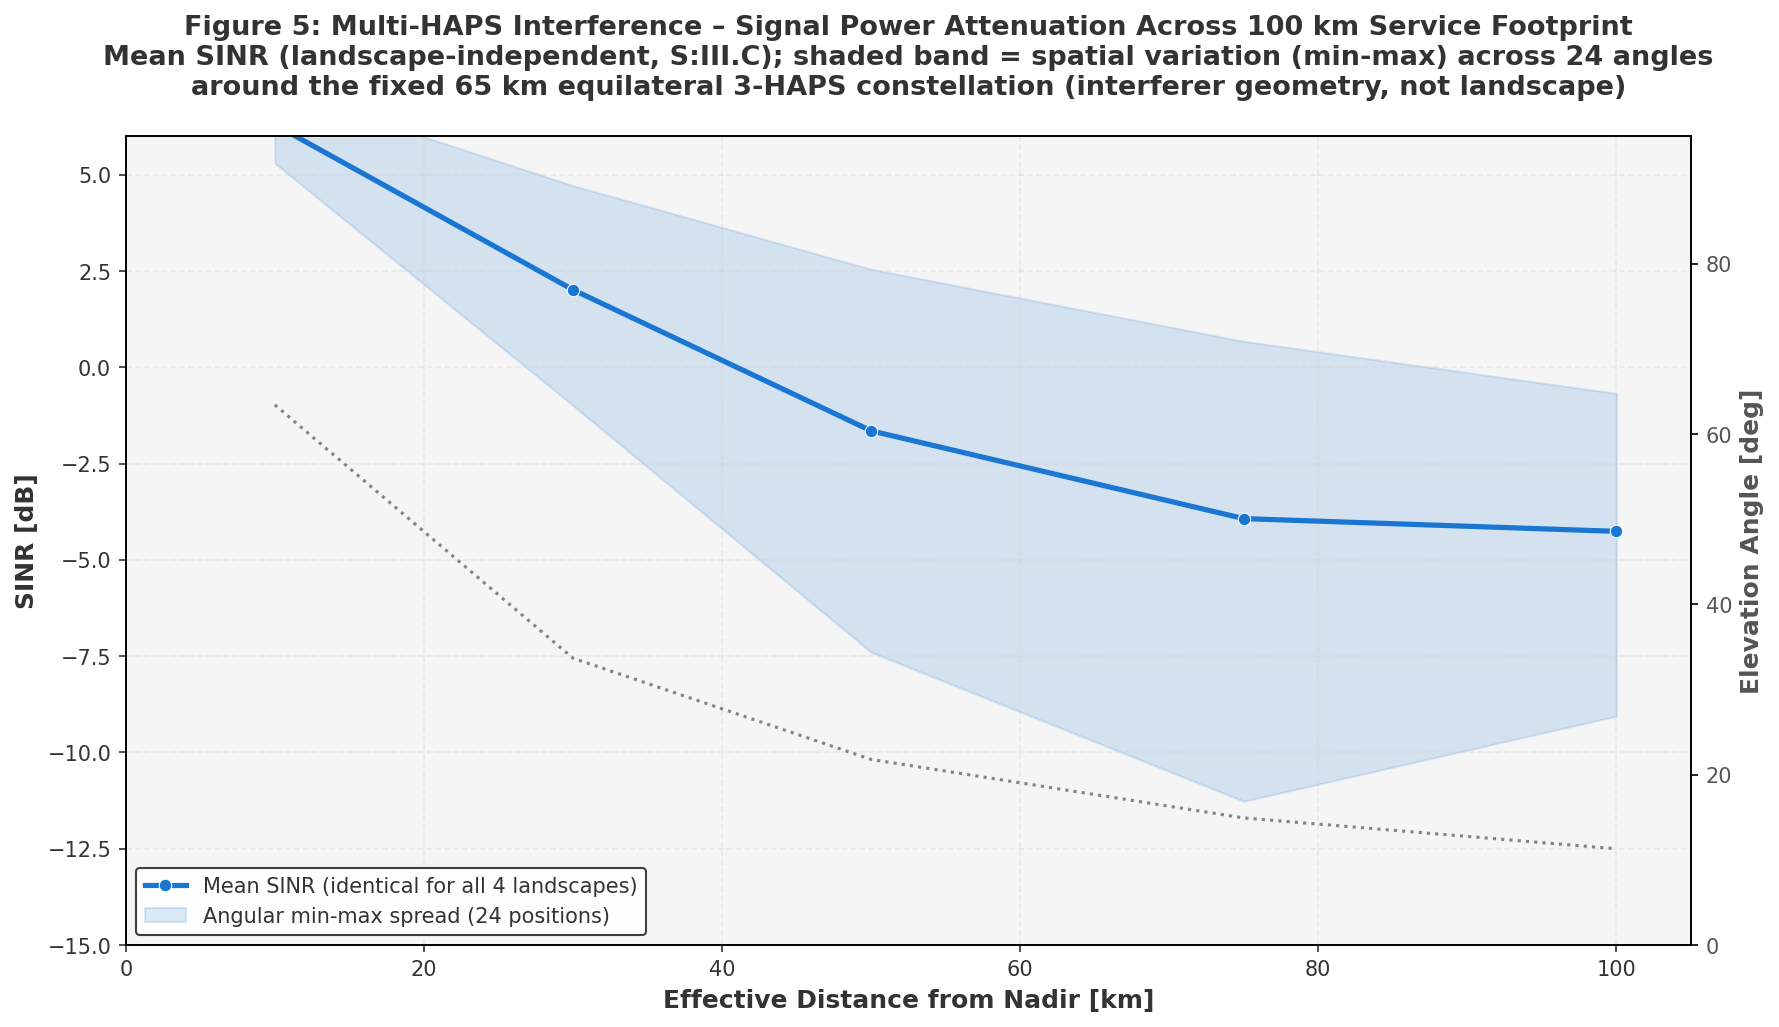
\includegraphics[width=\linewidth]{figure5_multi_haps_sinr_mean.png}
\end{column}
\begin{column}{0.45\textwidth}
\footnotesize
\begin{itemize}
  \item At a \textbf{fixed 50\,km radius}, SINR varies by
        \textbf{up to 9.94\,dB} depending on angular position relative to
        the two interfering HAPS.
  \item For comparison, simply \emph{doubling} the link distance only
        costs about 2--3\,dB -- so angular position affects SINR more
        than distance does.
  \item A simple ``always pick max-SINR'' rule cannot anticipate these
        angular patterns or adapt as weather and battery state change.
  \item \textbf{Conclusion:} a learned, real-time association policy is
        needed.
\end{itemize}
\end{column}
\end{columns}
\end{frame}

% ---------------------------------------------------------------
\begin{frame}{LSTM Rain-Attenuation Forecaster}
\begin{columns}[T]
\begin{column}{0.48\textwidth}
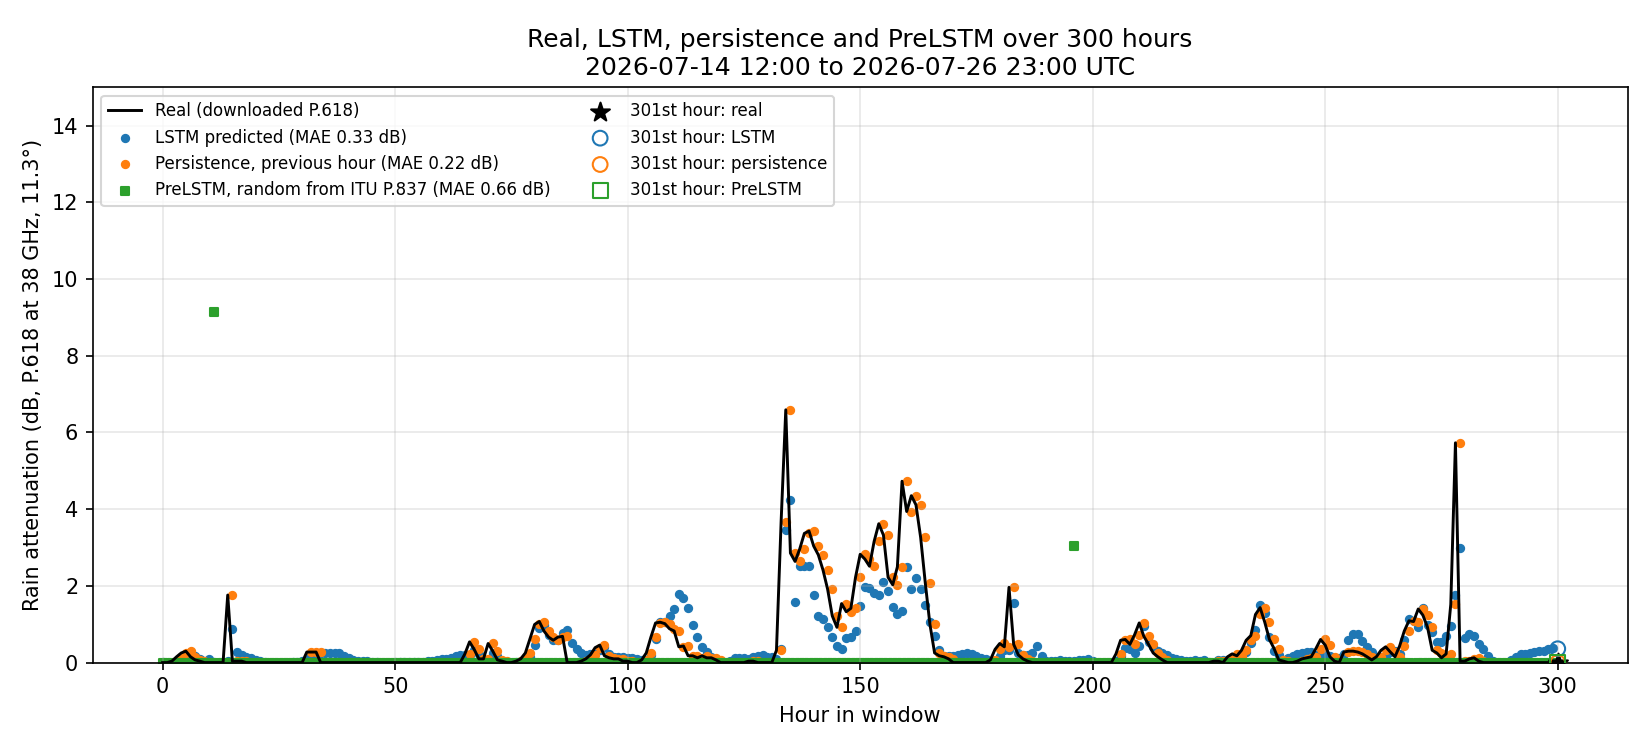
\includegraphics[width=\linewidth]{lstm_forecast_2026.png}
\vspace{2mm}
\footnotesize
\begin{itemize}\setlength{\itemsep}{2pt}
  \item DQN must decide at hour $t$ \emph{before} that hour's rain is
        observed $\Rightarrow$ needs a forecast.
  \item Evaluated \textbf{out-of-sample} (e.g.\ 2026 forecasts from a
        model trained on 2023--2025 data).
  \item In deployment this would be a \textbf{continuous, incremental}
        feed -- the model keeps updating as new weather data arrives.
\end{itemize}
\end{column}
\begin{column}{0.52\textwidth}
\footnotesize
\begin{itemize}\setlength{\itemsep}{2pt}
  \item LSTM predicts feeder (38\,GHz) rain attenuation up to
        \textbf{six hours ahead} from NASA POWER / METAR / ERA5 weather
        history for Delhi.
  \item More accurate than persistence at 4--6\,h (RMSE); all six
        forecast horizons feed the DQN's state.
  \item \textbf{Observation:} simply averaging the LSTM and persistence
        forecasts beats both alone on RMSE (0.511 vs.\ 0.645 / 0.530) --
        ensembling is a promising future direction.
\end{itemize}
\end{column}
\end{columns}
\end{frame}

% ---------------------------------------------------------------
\begin{frame}{DQN Association Agent: Problem Formulation}
\footnotesize
\textbf{Per-user MDP} -- each user independently chooses a platform; network
reward is computed after all assignments.
\vspace{2mm}

\begin{columns}[T]
\begin{column}{0.48\textwidth}
\begin{itemize}\setlength{\itemsep}{3pt}
  \item \textbf{State:} SINR to each platform, distance, battery SoC,
        rainfall, visibility, time-of-day, six LSTM rain forecasts.
  \item \textbf{Action:} $a_k \in \{0,\dots,5\}$ -- direct link to
        HAPS1--3, or relay through a UAV served by HAPS1--3.
\end{itemize}
\end{column}
\begin{column}{0.52\textwidth}
\begin{itemize}\setlength{\itemsep}{3pt}
  \item \textbf{Reward:} throughput (rain-derated) + fairness (Jain
        index) $-$ energy cost $-$ outage/degraded-service penalties
        $-$ low-battery penalty.
\end{itemize}
\vspace{2mm}
\begin{itemize}\setlength{\itemsep}{3pt}
  \item Custom Deep Q-Network implemented directly in PyTorch
        (\texttt{torch}/\texttt{torch.nn}).
  \item Trained on 400 rolling 24-hour episodes from 2024; evaluated on
        50 held-out 2025 days, five experiments (random seeds).
\end{itemize}
\end{column}
\end{columns}
\end{frame}

% ---------------------------------------------------------------
\begin{frame}{Results: Policy Comparison}
\footnotesize
\begin{table}
\centering
\begin{tabularx}{\linewidth}{|>{\raggedright\arraybackslash}X|>{\centering\arraybackslash}X|>{\centering\arraybackslash}X|>{\centering\arraybackslash}X|}
\hline
\textbf{Policy} & \textbf{Reward/step} & \textbf{Jain} & \textbf{Outage /50} \\
\hline
Random (six actions) & $-40.5\,(1.7)$ & $0.563\,(0.007)$ & $16.5\,(0.4)$ \\
\hline
Max-SINR (direct only) & $-14.5\,(2.1)$ & $0.866\,(0.002)$ & $0.9\,(0.2)$ \\
\hline
Max-throughput (six actions) & $-3.8\,(1.7)$ & $\mathbf{0.988}\,(0.000)$ & $\mathbf{0.0}\,(0.0)$ \\
\hline
\textbf{LSTM + DQN} & $\mathbf{+1.4}\,(1.0)$ & $0.981\,(0.006)$ & $\mathbf{0.0}\,(0.0)$ \\
\hline
\end{tabularx}
\end{table}
\begin{itemize}
  \item Mean $\pm$ std.\ dev.\ over five experiments, 50 held-out 2025 days.
  \item DQN has the \textbf{highest reward}, zero outage, and fairness
        statistically indistinguishable from max-throughput.
  \item Max-SINR assumes perfect SINR knowledge and cannot use the relay
        actions -- the DQN doesn't need either assumption.
  \item Max-throughput also assumes perfect, instantaneous knowledge of
        every option's SINR/capacity, and has no memory, battery, or
        fairness awareness -- a theoretical upper bound, not a
        deployable policy.
\end{itemize}
\end{frame}

% ---------------------------------------------------------------
\begin{frame}{Results: Stability Across Experiments}
\begin{columns}[T]
\begin{column}{0.48\textwidth}
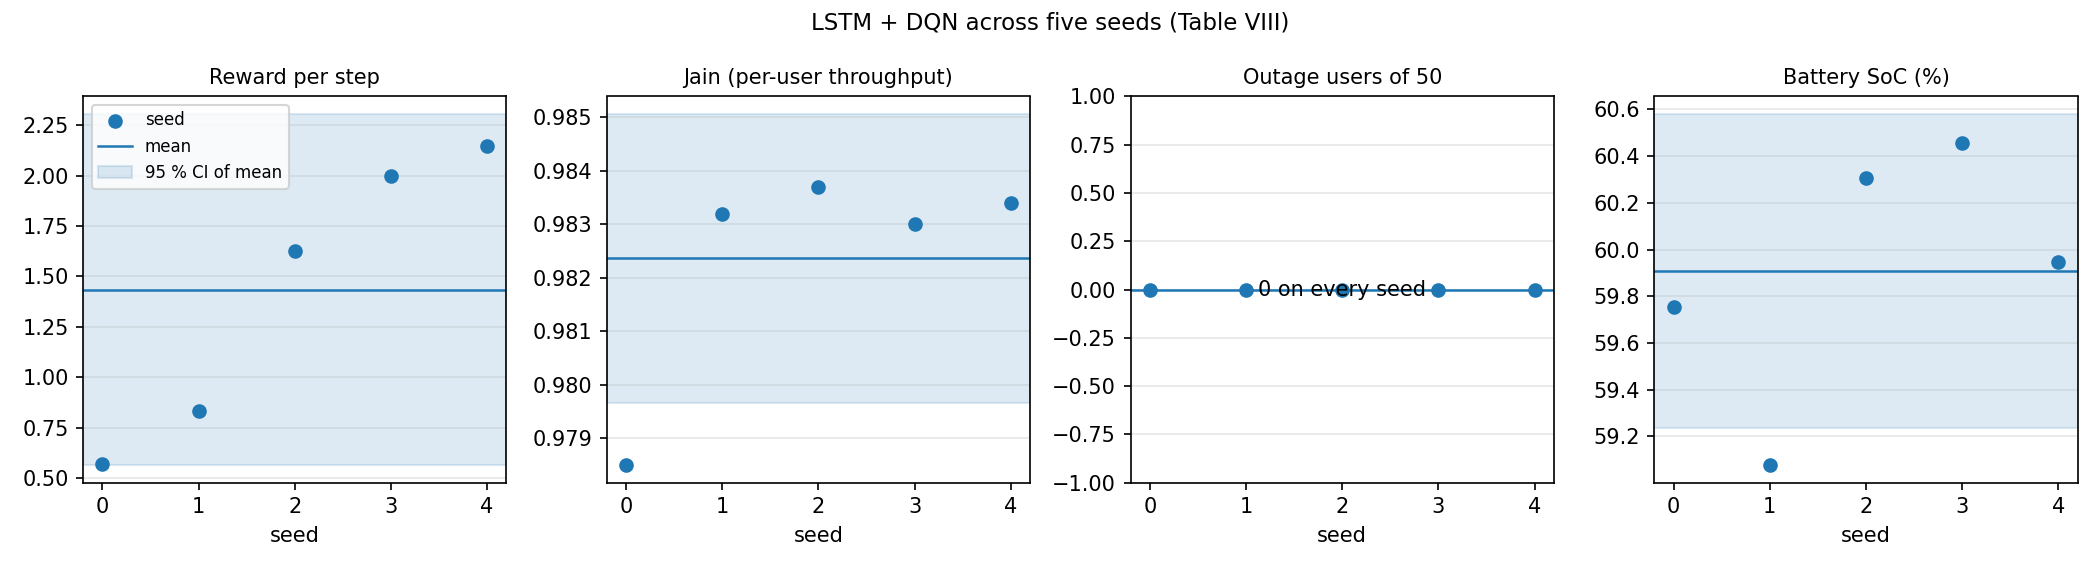
\includegraphics[width=\linewidth]{seed_stats.png}
\vspace{2mm}
\scriptsize
\textbf{LSTM + DQN, five independent seeds} (dot = one training run;
line = mean; band = 95\% CI \emph{of the mean}):
\begin{itemize}\setlength{\itemsep}{0pt}
  \item Reward/step: $+1.40 \pm 0.96$ \\ (95\% CI $[0.21, 2.59]$)
  \item Jain fairness: $0.981 \pm 0.006$
  \item Outage: $0.0 \pm 0.0$ (every seed, every day)
  \item Battery SoC: $59.96 \pm 0.59\,\%$
\end{itemize}
\end{column}
\begin{column}{0.52\textwidth}
\scriptsize
\textbf{CI vs.\ spread:} the shaded band is \emph{not} ``most runs land
here'' -- it narrows with more seeds even if run-to-run variability
($\pm0.96$) stays the same. It shows how precisely the \emph{true mean}
is known from only 5 runs.

\vspace{2mm}
\textbf{On the seed axis:} seed is just a run label (0--4 are RNG seeds,
not a meaningful scale) -- any apparent rise with seed number is
run-to-run noise, not a real trend; e.g.\ Jain and battery SoC don't
follow the same order as reward.

\vspace{2mm}
\textbf{Takeaway:} zero outage and tight fairness/SoC variance across
all 5 seeds show the policy is \textbf{reliably learned}, not a lucky
single run.
\end{column}
\end{columns}
\end{frame}

% ---------------------------------------------------------------
\begin{frame}{Results: Statistical Significance}
\begin{columns}[T]
\begin{column}{0.42\textwidth}
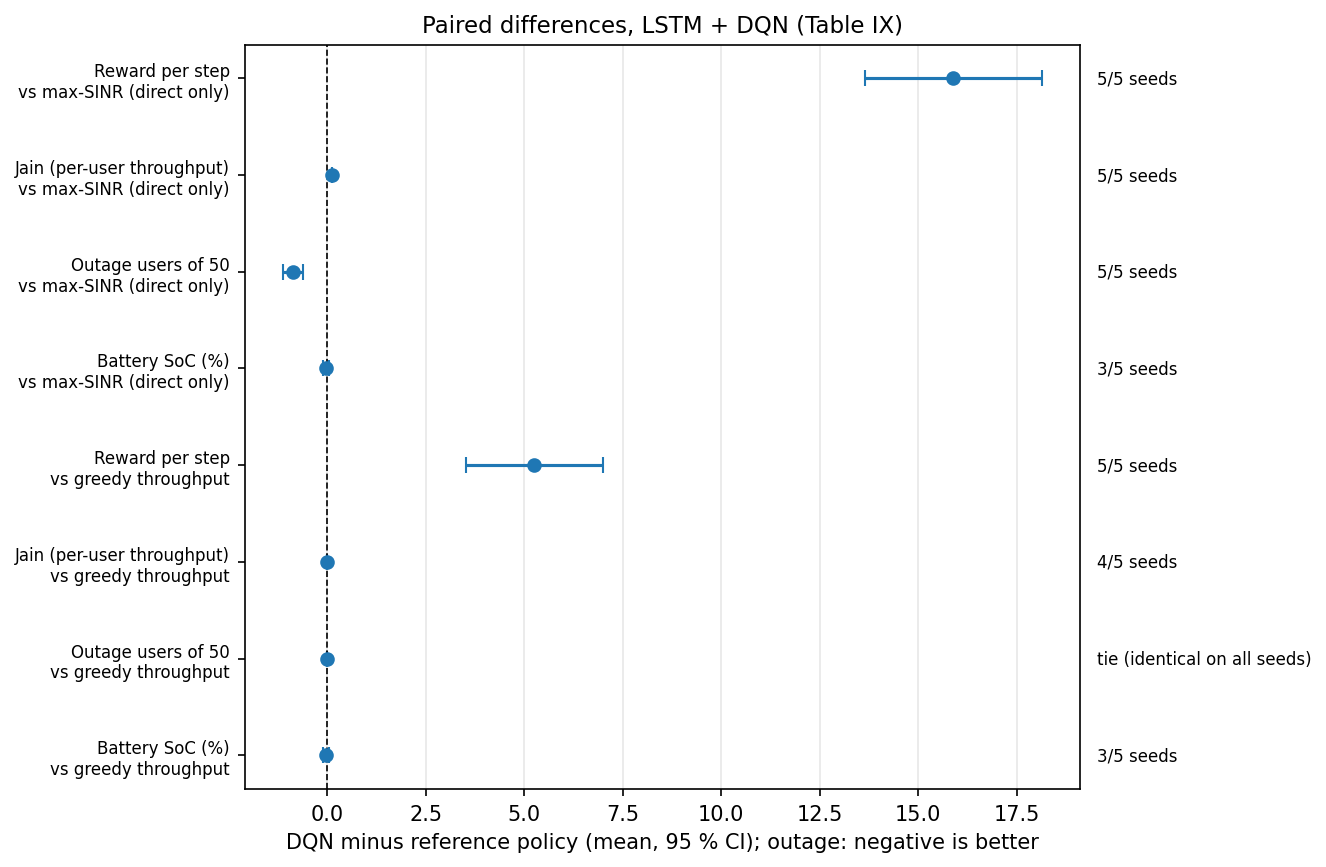
\includegraphics[width=\linewidth]{paired_forest.png}
\end{column}
\begin{column}{0.58\textwidth}
\scriptsize
Paired differences, LSTM+DQN minus baseline (per experiment, 50 days each).
Whiskers crossing 0 = not significant.

\vspace{1mm}
\textbf{vs.\ Max-SINR (direct links only):}
\begin{itemize}\setlength{\itemsep}{0pt}
  \item Reward: $+15.87$ ($p<0.001$) -- \textbf{significant}, 5/5
  \item Jain: $+0.115$ ($p<0.0001$) -- \textbf{significant}, 5/5
  \item Outage: $-0.87$ ($p=0.0007$) -- \textbf{significant}, 5/5
  \item Battery SoC: $+0.03$ ($p=0.44$) -- not significant (tie)
\end{itemize}

\vspace{1mm}
\textbf{vs.\ Max-throughput (greedy, all 6 actions):}
\begin{itemize}\setlength{\itemsep}{0pt}
  \item Reward: $+5.17$ ($p=0.001$) -- \textbf{significant}, 5/5
  \item Jain: $-0.007$ ($p=0.07$) -- not significant (tie)
  \item Outage: $0$ -- tie, identical on every seed
  \item Battery SoC: $\approx 0$ -- not significant (tie)
\end{itemize}

\vspace{1mm}
\textbf{Takeaway:} DQN beats Max-SINR on 3 of 4 metrics. Against the
stronger, information-privileged Max-throughput baseline, it wins only
on reward -- and \emph{ties, never loses}, on fairness, outage, and
battery.
\end{column}
\end{columns}
\end{frame}

% ---------------------------------------------------------------
\begin{frame}{Conclusion and Future Work}
\scriptsize
\textbf{Channel model.} Spatial SINR heterogeneity (up to 9.94\,dB at
fixed 50\,km) dominates service-link quality; backhaul remains
noise-limited. \quad
\textbf{Relay path.} HAPS$\to$UAV$\to$UE outperforms the direct link at
every distance tested (11.1 vs.\ 2.7\,bits/s/Hz at nadir); keeping the
UAV near nadir (high elevation) on the 38\,GHz feeder hop limits rain
and scintillation losses, both of which grow sharply as the slant path
lengthens at low elevation. \quad
\textbf{Learned association.} The LSTM-fed DQN beats max-throughput and
max-SINR on reward, with zero outage and no significant fairness loss.

\vspace{2mm}
\textbf{Future work:}
\begin{itemize}\setlength{\itemsep}{0pt}
  \item Learn \emph{when} relaying is worthwhile as a function of user distance.
  \item Model movement of the HAPS and UAV platforms.
  \item Consider more UAVs, including UAV selection.
  \item Extend the LSTM forecast to neighbouring regions (e.g.\ ConvLSTM
        on gridded reanalysis data, or a spatio-temporal GNN if future
        sites are irregularly placed).
  \item Adapt to changing HAPS roles (shift a node between service and
        interferer based on its distance to the gateway).
  \item Jointly optimize UAV/HAPS positioning across both roles a node
        could play at once -- serving node for its own users, interferer
        for the other HAPS' users -- rather than each in isolation.
  \item Consider beamforming between HAPS and Gateway.
  \item Explore forecast ensembling (e.g.\ LSTM + persistence averaging
        already improved RMSE in our initial check, slide~5).
\end{itemize}

\vspace{2mm}
\centering \large Thank you -- Questions?
\end{frame}

\end{document}
